\documentclass[xcolor=x11names,compress,aspectratio=169]{beamer}
%\documentclass[xcolor=x11names,compress,aspectratio=43]{beamer}

%% General document %%%%%%%%%%%%%%%%%%%%%%%%%%%%%%%%%%
\usepackage{graphicx}
\usepackage{tikz}
\usepackage{amsmath}
\usepackage{amssymb}
\usepackage[utf8]{inputenc}
\usepackage{textpos}
\usepackage{booktabs}
\usepackage{listings}
\usepackage{auto-pst-pdf}

\usetikzlibrary{decorations.fractals, calc}
%%%%%%%%%%%%%%%%%%%%%%%%%%%%%%%%%%%%%%%%%%%%%%%%%%%%%%

%% Beamer Layout %%%%%%%%%%%%%%%%%%%%%%%%%%%%%%%%%%
\useoutertheme[subsection=false,shadow]{miniframes}
\useinnertheme{default}
%\usefonttheme{serif}
\usepackage{palatino}
\setbeamerfont{title like}{shape=\scshape}
\setbeamerfont{frametitle}{shape=\scshape}
\beamertemplatenavigationsymbolsempty


% Uncomment this line, if you want frame numbers on your slides
% (I disabled them since I had the progress bar at the header)
%\setbeamertemplate{footline}[frame number]

\definecolor{fmiBlue}{RGB}{11,128,145} % FSU Faculty blue
\definecolor{evbc}{RGB}{50,167,132} % EVBC Green
\definecolor{bgGray}{RGB}{230,230,230} % some gray if needed


\setbeamercolor*{upper separation line head}{bg=Snow4} %Snow4 comes from the x11names option of xcolor
%\setbeamercolor*{lower separation line head}{bg=evbc}  % obsolete - there is now a cool progress bar 
\setbeamercolor*{normal text}{fg=black,bg=white} 
\setbeamercolor*{alerted text}{fg=red} 
\setbeamercolor*{example text}{fg=black} 
\setbeamercolor*{structure}{fg=black} 
 
\setbeamercolor*{palette tertiary}{fg=black,bg=black!10} 
\setbeamercolor*{palette quaternary}{fg=black,bg=black!10} 

%%%%%%%%%%%%%%%%%%%%%%%%%%%%%%%%%%%%%%%%%%%%
% IMPORTANT
% Kevin:
% Currently the FMI blue (the light uni blue) is here.
% If you want for example the evbc green, you'd have to
% change the colors here. I will put this in a nice function
% at some point.
\setbeamercolor{title}{fg=evbc}
\setbeamercolor{structure}{fg=evbc}
\setbeamercolor{frametitle}{fg=evbc}
\setbeamercolor{block title}{fg=evbc, bg=bgGray}
\setbeamercolor{block title example}{fg=evbc}
\setbeamercolor{enumerate item}{fg=evbc}
\setbeamercolor{itemize item}{fg=evbc}
\setbeamercolor{item projected}{bg=evbc}

\setbeamerfont{block title}{size=\small}
\setbeamerfont{block body}{size=\scriptsize}

% Use those if you want. Just some shortcuts for 
% columns. Personally, I use minipages nowadays.
\renewcommand{\(}{\begin{columns}}
\renewcommand{\)}{\end{columns}}
\newcommand{\<}[1]{\begin{column}{#1}}
\renewcommand{\>}{\end{column}}

% Kevin:
% This is used for the code examples in the document.
% If used, set the frame option to 'fragile' (!!!)
\lstset{
	language=sh, 
	numbers=left, 
	numberstyle=\tiny\color{gray}, 
	backgroundcolor=\color{bgGray}, 
	basicstyle=\scriptsize\ttfamily,
	commentstyle=\tiny\color{Green4},
	keywordstyle=\color{Blue3},
	escapeinside=@@
}

% Kevin
% Appendix page number fix. More like an ugly hack.
% I was never able to create a "nice" appendix command, however, this one here works fine.
\newcommand{\beginbackup}{
   \newcounter{framenumbervorappendix}
   \setcounter{framenumbervorappendix}{\value{framenumber}}
}
\newcommand{\backupend}{
   \addtocounter{framenumbervorappendix}{-\value{framenumber}}
   \addtocounter{framenumber}{\value{framenumbervorappendix}} 
}

%%%%%%%%%%%%%%%%%%%%%%%%%%%%%%%%%%%%%%%%%%%%%%%%%%
% Kevin: Change this, if you want.
\graphicspath{{figures/}}
%

% Kevin:
% I used this slides for subsections a long time ago, however, at some point I figured that it is nicer to have those slides
% at the beginning of each section. Use this extra slides to give a short summary of the previous talk.
\AtBeginSection[]{
  \begin{frame}
  \vfill
  \centering
  \begin{beamercolorbox}[sep=8pt,center,shadow=true,rounded=true]{title}
    \usebeamerfont{title}\insertsection\par%
  \end{beamercolorbox}
  \vfill
  \end{frame}
}


% Kevin:
% small macro, used to build the progress bar
\def\insertframeratio{%
    \pgfmathparse{\insertframenumber/\inserttotalframenumber}%
}
%%%%%%%%%%%%%%%%%%%%%%%%%%
% Kevin:
% This is the progress bar in the headline.
% Change the textcolor if needed, change the width to 2pt if wanted
\addtobeamertemplate{headline}{}{%
  \insertframeratio
  \edef\myvar{\pgfmathresult}
  %\textcolor{evbc}{\rule{\myvar \paperwidth}{1pt}}
  \textcolor{evbc}{\rule{\paperwidth}{1pt}}
}

%%%%%%%%%%%%%%%%%%%%%%%%%%%
% Kevin
% This adds the FSU Logo to the
% bottom left. Changing the logo is easy
% adding a second logo (e.g. the evbc) is tricky
\addtobeamertemplate{footline}{}{%
\begin{textblock*}{100mm}(1em,-3.5em)

\includegraphics[scale=0.4]{evbc_cmyk.pdf}
\end{textblock*} 
\begin{textblock*}{100mm}(73em,-1em) 
\insertframenumber/\inserttotalframenumber
\end{textblock*}
}

%% Kevin:
%% I used this in order to show two logos at the same time.
%% as you can see, it is quite tricky in terms of positioning 
%% and size, but a nice try-and-error session usually
%% works out.
%\addtobeamertemplate{footline}{}{%
%\begin{textblock*}{100mm}(0.5em,-5em)
%
\includegraphics[scale=0.5]{figures/evbc_cmyk.pdf}
%\end{textblock*}
%\begin{textblock*}{100mm}(11em,-3em)
%
\includegraphics[scale=0.025]{fsu_logo.jpg}
%\end{textblock*}
%}


% Kevin:
% Well, fill this out as needed
%\title{Theoretical and practical metagenomic approaches to viral discovery}
%\subtitle{}
%\author{Kevin Lamkiewicz, Manja Marz}
%\date{27.09.2018\\[1em]RNA Bioinformatics and High-Throughput Analysis\\[1em]Friedrich Schiller University Jena}
%\date{xx.xx.2018\\RNA Bioinformatics and High-Throughput Analysis\\[2em]
\includegraphics[scale=0.05]{fsu_logo.jpg}}



\title{Theoretical and practical metagenomic approaches to viral discovery}
\subtitle{Practical Session: ViennaRNA for RNA-RNA Interactions}
\author{Kevin Lamkiewicz, Manja Marz}
\date{24.10.2019\\[1em]European Virus Bioinformatics Center}

\begin{document}

\begin{frame}
  \maketitle
\end{frame}

\begin{frame}[c]{Why RNA-RNA Interactions?}
  \pause
  \begin{figure}[htbp]
    \centering
    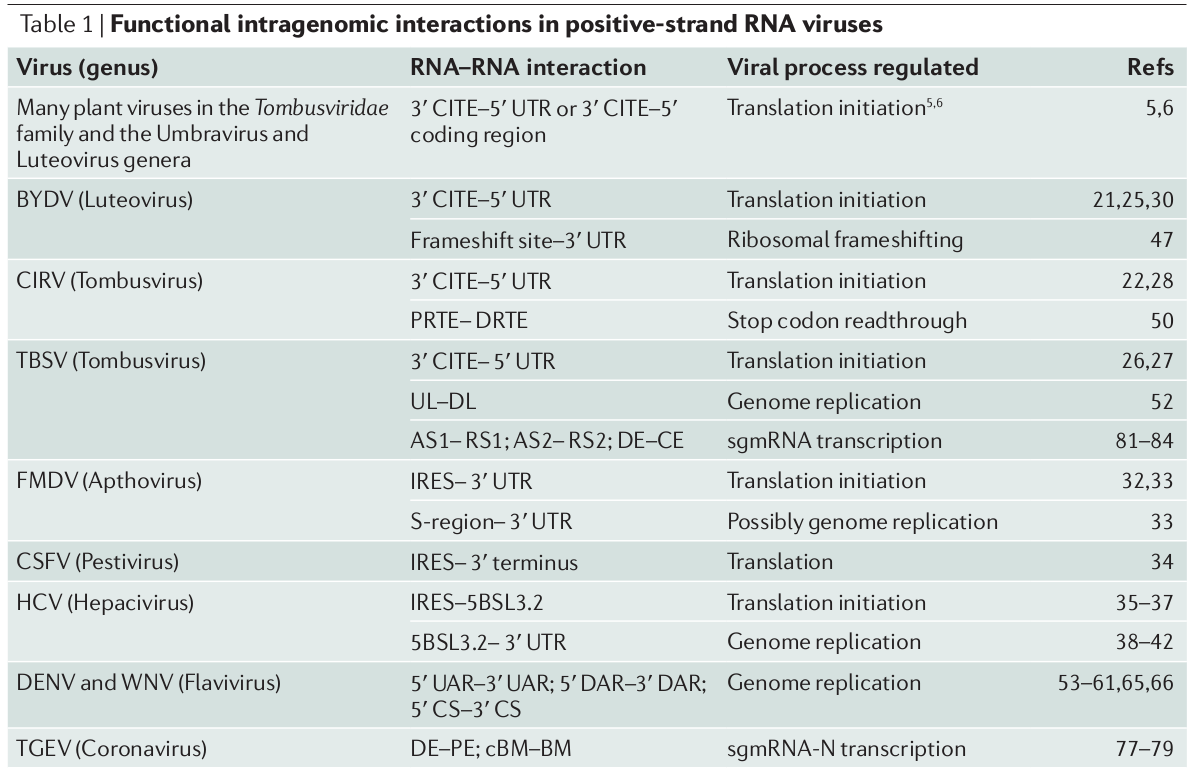
\includegraphics[width=0.7\textwidth]{lri_review.png}\\
    {\tiny Beth L. Nicholson and K. Andrew White (2014) "Functional long-range RNA-RNA interactions in positive-strand RNA viruses.",\\
     Nature Reviews Microbiology volume 12, pages 493–504}
  \end{figure}
\end{frame}

\section[Sequences]{Interactions for single sequences}


\begin{frame}[c, fragile]\frametitle{RNAcofold}
  \begin{lstlisting}
# RNAcofold works like RNAfold, but allows to specify two RNA sequences.
# These sequences are then allowed to form a dimer structure. In order
# to calculate the hybrid structure, it is necessary to concatenate the
# two RNA sequence, using & as a separator.

$> RNAcofold [OPTIONS] < sequences.fasta > sequences.cofold

# >seq1
# AUGGCAUCGACA
# >seq2
# UGUCGAAUCCAA

# RNAcofold Input:
# AUGGCAUCGACA&UGUCGAAUCCAA
  \end{lstlisting}
\end{frame}

\begin{frame}[c]\frametitle{RNAcofold}
  \begin{minipage}[c]{0.4\textwidth}
  \begin{figure}
    \centering
    
\includegraphics[height=0.75\textheight]{cofold_simple.pdf}
  \end{figure}
\end{minipage}\hfill\begin{minipage}[c]{0.55\textwidth}
  \begin{itemize}
    \item First sequence is colored green
    \item Second sequence is colored red\\[3em]
  \end{itemize}
\end{minipage}
\end{frame}

\begin{frame}[c, fragile]\frametitle{RNAcofold with partition function}
  \begin{lstlisting}
# We calculated the MFE structure of the interacting molecules (RNA dimer).
# RNAcofold also has the -p parameter implemented. 

$> RNAcofold -p < sequences.fasta > sequences.cofold

  \end{lstlisting}
  \vspace{4em}
  \uncover<2->{
    We can use \texttt{relplot.pl} on the PostScript files as well,
    but it looks a bit... weird.
  }
\end{frame}

\begin{frame}[c]\frametitle{RNAcofold with partition function}
  \begin{figure}
    \centering
    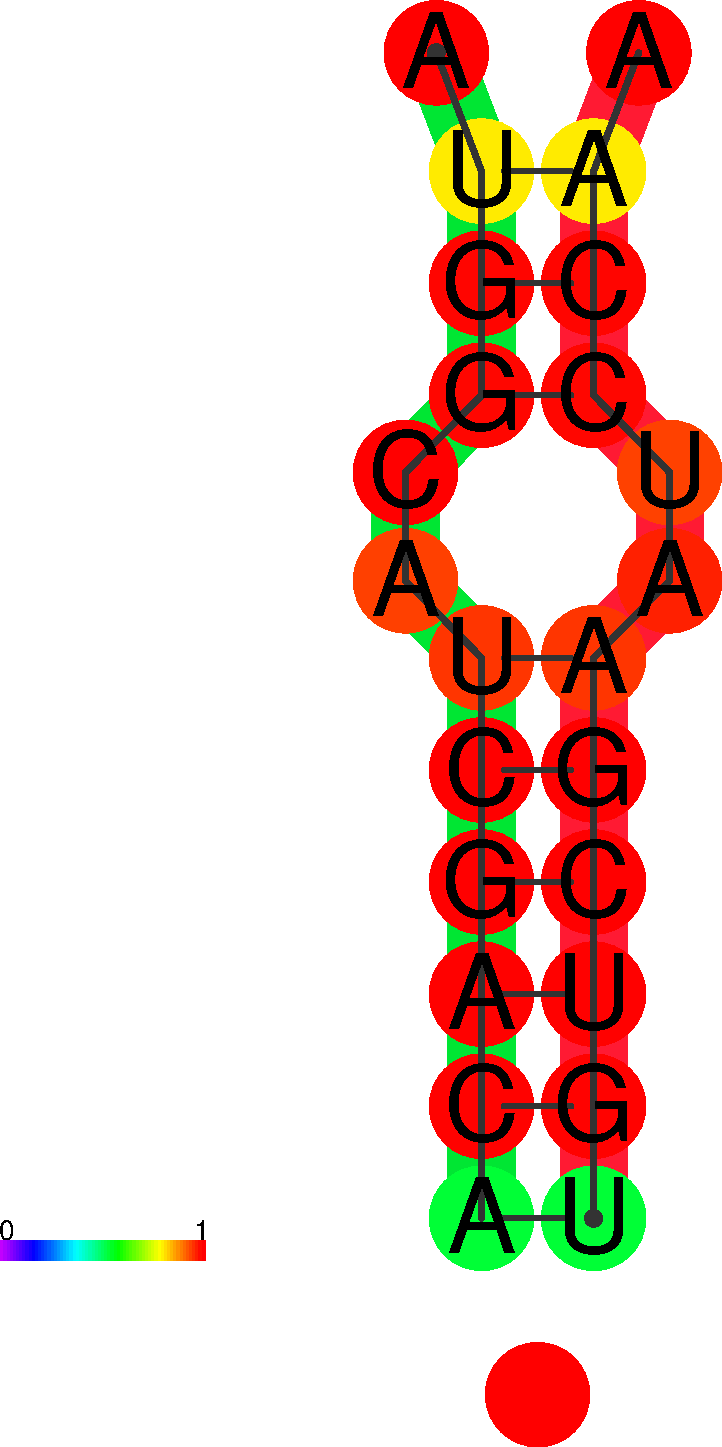
\includegraphics[height=0.75\textheight]{cofold_simple_part.pdf}
  \end{figure}
\end{frame}


\begin{frame}[c,fragile]{AA, AB, BB}
    \begin{lstlisting}
  # Until now, we just looked at the heterodimer of the two sequences.
  # But how do the molecules behave individually?
  
  $> RNAcofold -a < sequences.fasta > sequences.cofold
    \end{lstlisting}
    \vspace{4em}
    \uncover<2->{
      The AA and BB dimer describe the MFE structure of two RNA molecules of
      sequence one and sequence two, respectively.
    }
\end{frame}

\begin{frame}[c, fragile]\frametitle{RNAduplex}
  \begin{lstlisting}
# RNAduplex is very similar to RNAcofold. Actually,
# it is a special case of RNAcofold, where only inter-molecular
# base pairs are allowed.

$> RNAduplex [OPTIONS] < sequences.fasta > sequences.duplex
@\pause@
# Alternative:
# RNAcofold -C < sequences_constrained.fasta
# sequences_constrained.fasta
# UAGCUAGCAUGCAUCGACGAU&CGAUGCAUGCAUGCAUGCAUC
# <<<<<<<<<<<<<<<<<<<<<&>>>>>>>>>>>>>>>>>>>>>
  \end{lstlisting}
\end{frame}


\section[Alignments]{Co-Folding with MSAs}

\begin{frame}[c,fragile]{RNAaliduplex}
  \begin{overlayarea}{\linewidth}{\textheight}
  \uncover<2->{
  \begin{block}{Not much implemented...}
    Unfortunately, ViennaRNA does not provide many possibilities for alignment-based co-folding 
    analyses. Indeed, only the alignment version of \texttt{RNAduplex} is implemented in \texttt{RNAaliduplex}.
  \end{block}
  } \vspace{5em} 
  \begin{onlyenv}<3>
    
\begin{lstlisting}
RNAaliduplex [OPTIONS] <file1.aln> <file2.aln>
@\pause@
# RNAaliduplex expects two input files (both CLUSTAL alignments)
# and predicts optimal and suboptimal binding sites. 
# However, only inter-molecular base pairs are taken into account.
\end{lstlisting}
\end{onlyenv}
\end{overlayarea}
\end{frame}

\begin{frame}[c, fragile]{Alignment-based intra-molecular base pairs?}
  \uncover<2->{
  \begin{block}{What would you do?}
    Discuss, play around, try to make some examples - I will go around and answer questions, discuss your ideas
    and help you as good as I can.
  \end{block}
  }
\end{frame}


\begin{frame}[c, fragile]{Alignment-based intra-molecular base pairs!}
  \uncover<2->{
  \begin{block}{Different ways to do it}
    Most commonly, you'd want to do the following:
    \begin{enumerate}
      \item Extract your sequences and align them individually
      \item Merge the alignments, use \texttt{'NNNNN'} as a separator
      \item Apply \texttt{RNAalifold} on the alignment
    \end{enumerate}
  \end{block}
  }
\end{frame}

\section[LRIs]{Long-Range Interactions}


\begin{frame}[c]{We remember...}
  \pause
  \begin{figure}[htbp]
    \centering
    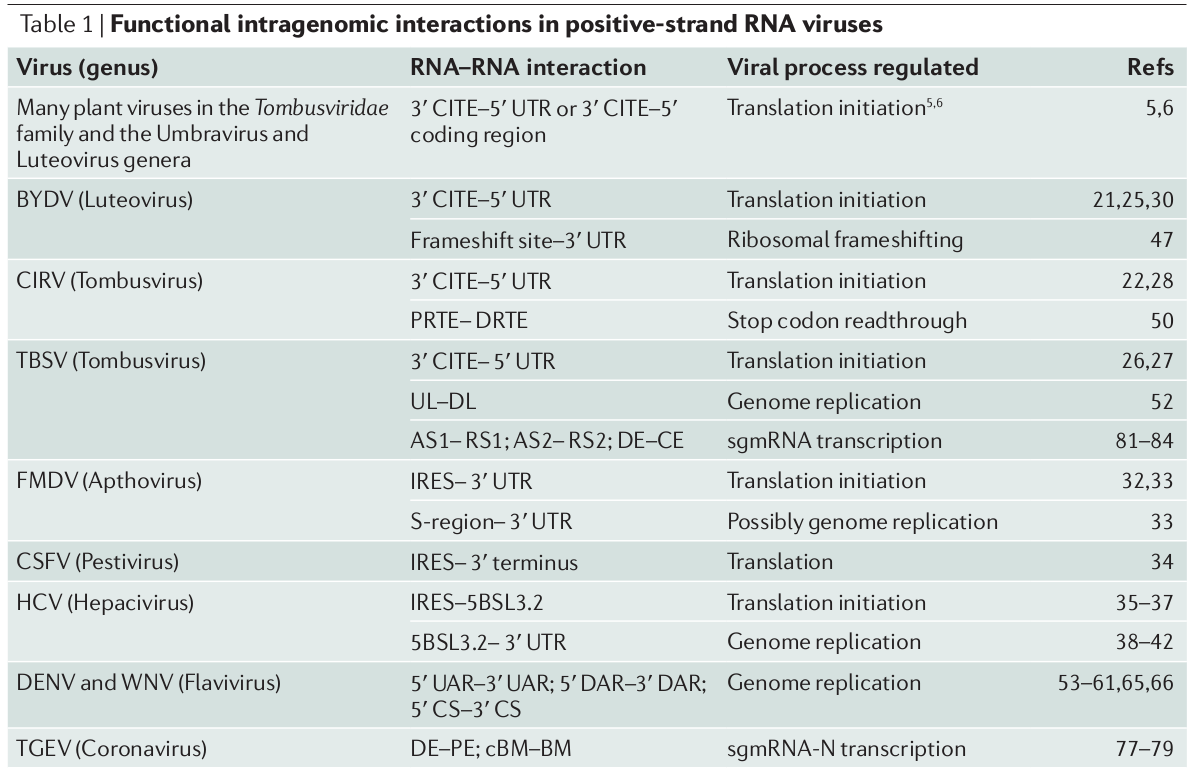
\includegraphics[width=0.7\textwidth]{lri_review.png}\\
    {\tiny Beth L. Nicholson and K. Andrew White (2014) "Functional long-range RNA-RNA interactions in positive-strand RNA viruses.",\\
     Nature Reviews Microbiology volume 12, pages 493–504}
  \end{figure}
\end{frame}


\begin{frame}[c]\frametitle{Why LRIs?}
  \begin{itemize}
    \item Interaction spans distances between a few hundred and several thousands of nucleotides
    \item few are described in positive stranded RNA viruses
    \item often located in loop regions (bulges, hairpins, ...)\\
    \uncover<2->{
    $\Rightarrow$ pseudo-knots!
    }
  \end{itemize}
 \end{frame}

\begin{frame}[c]\frametitle{RNA-RNA interactions are crucial for RNA viruses}
  \begin{columns}
  \column{0.6\textwidth}
  \begin{overlayarea}{\linewidth}{\textheight}
  \only<1>{
  \centering
  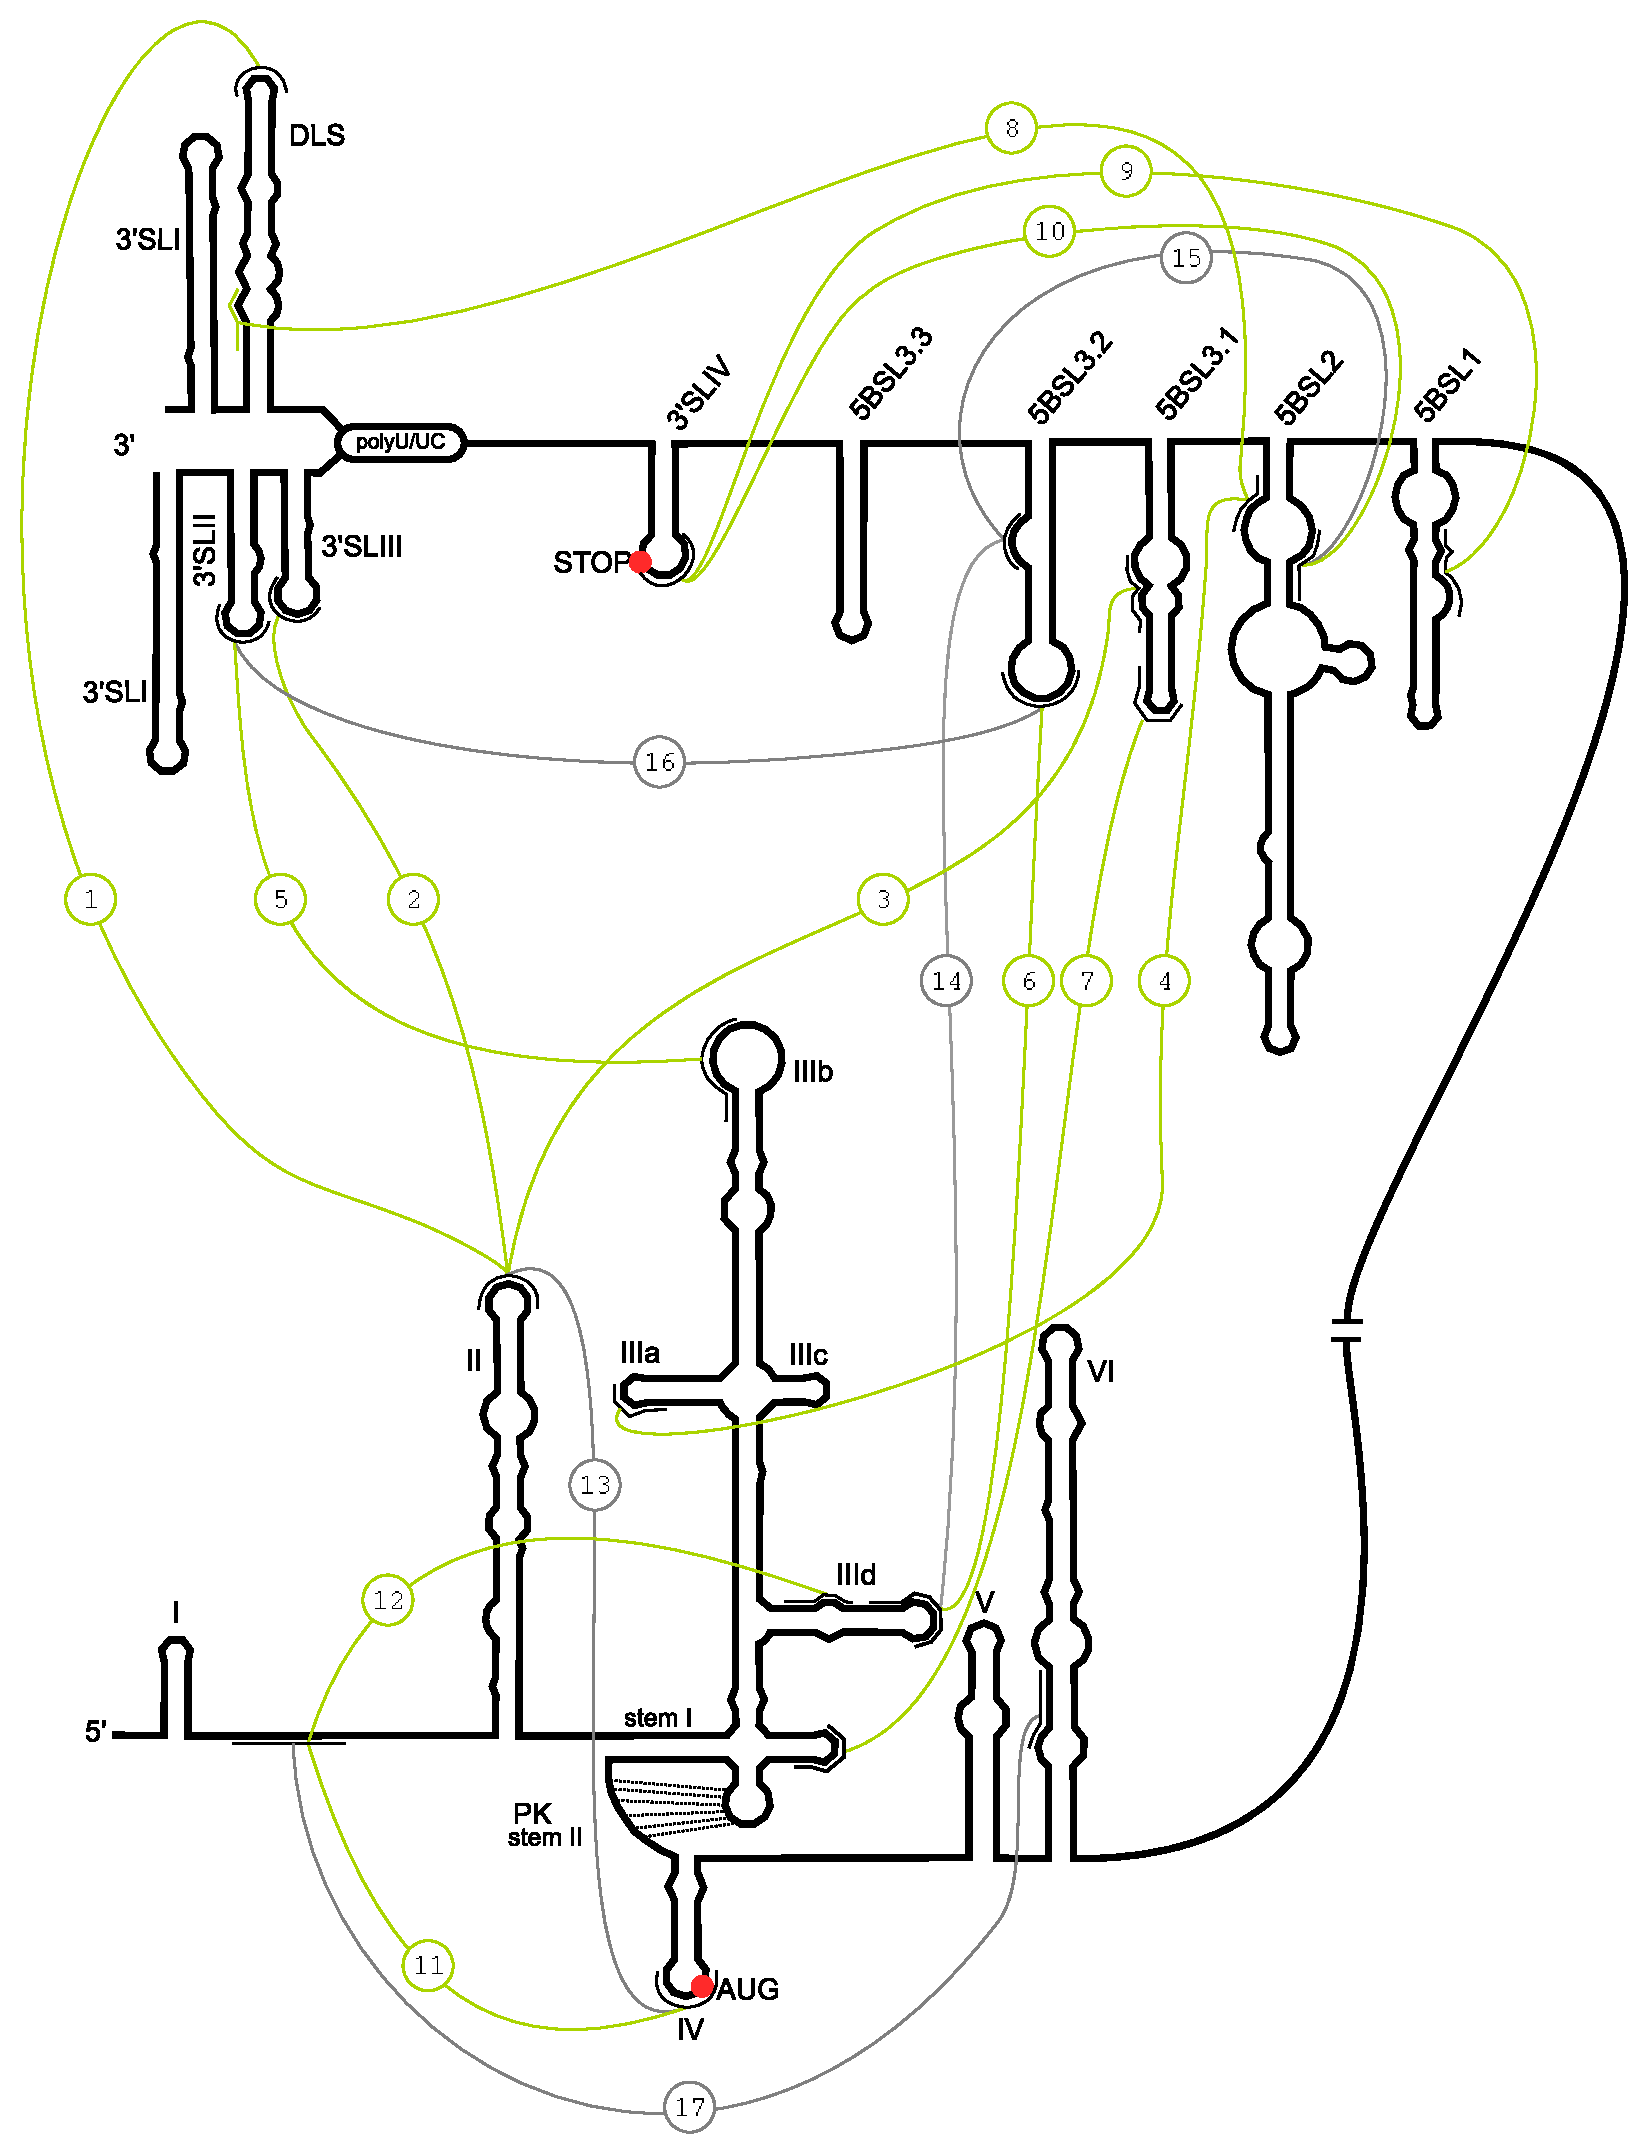
\includegraphics[height=0.7\textheight]{figures/long_range_hcv.pdf}\\%
  \tiny{Fricke, M.~\textit{et al.}~(2015).~Conserved RNA secondary structures and long-range interactions in hepatitis C viruses. RNA, http://doi.org/10.1261/rna.049338.114}%
  } 
  \only<2> {
  \centering
  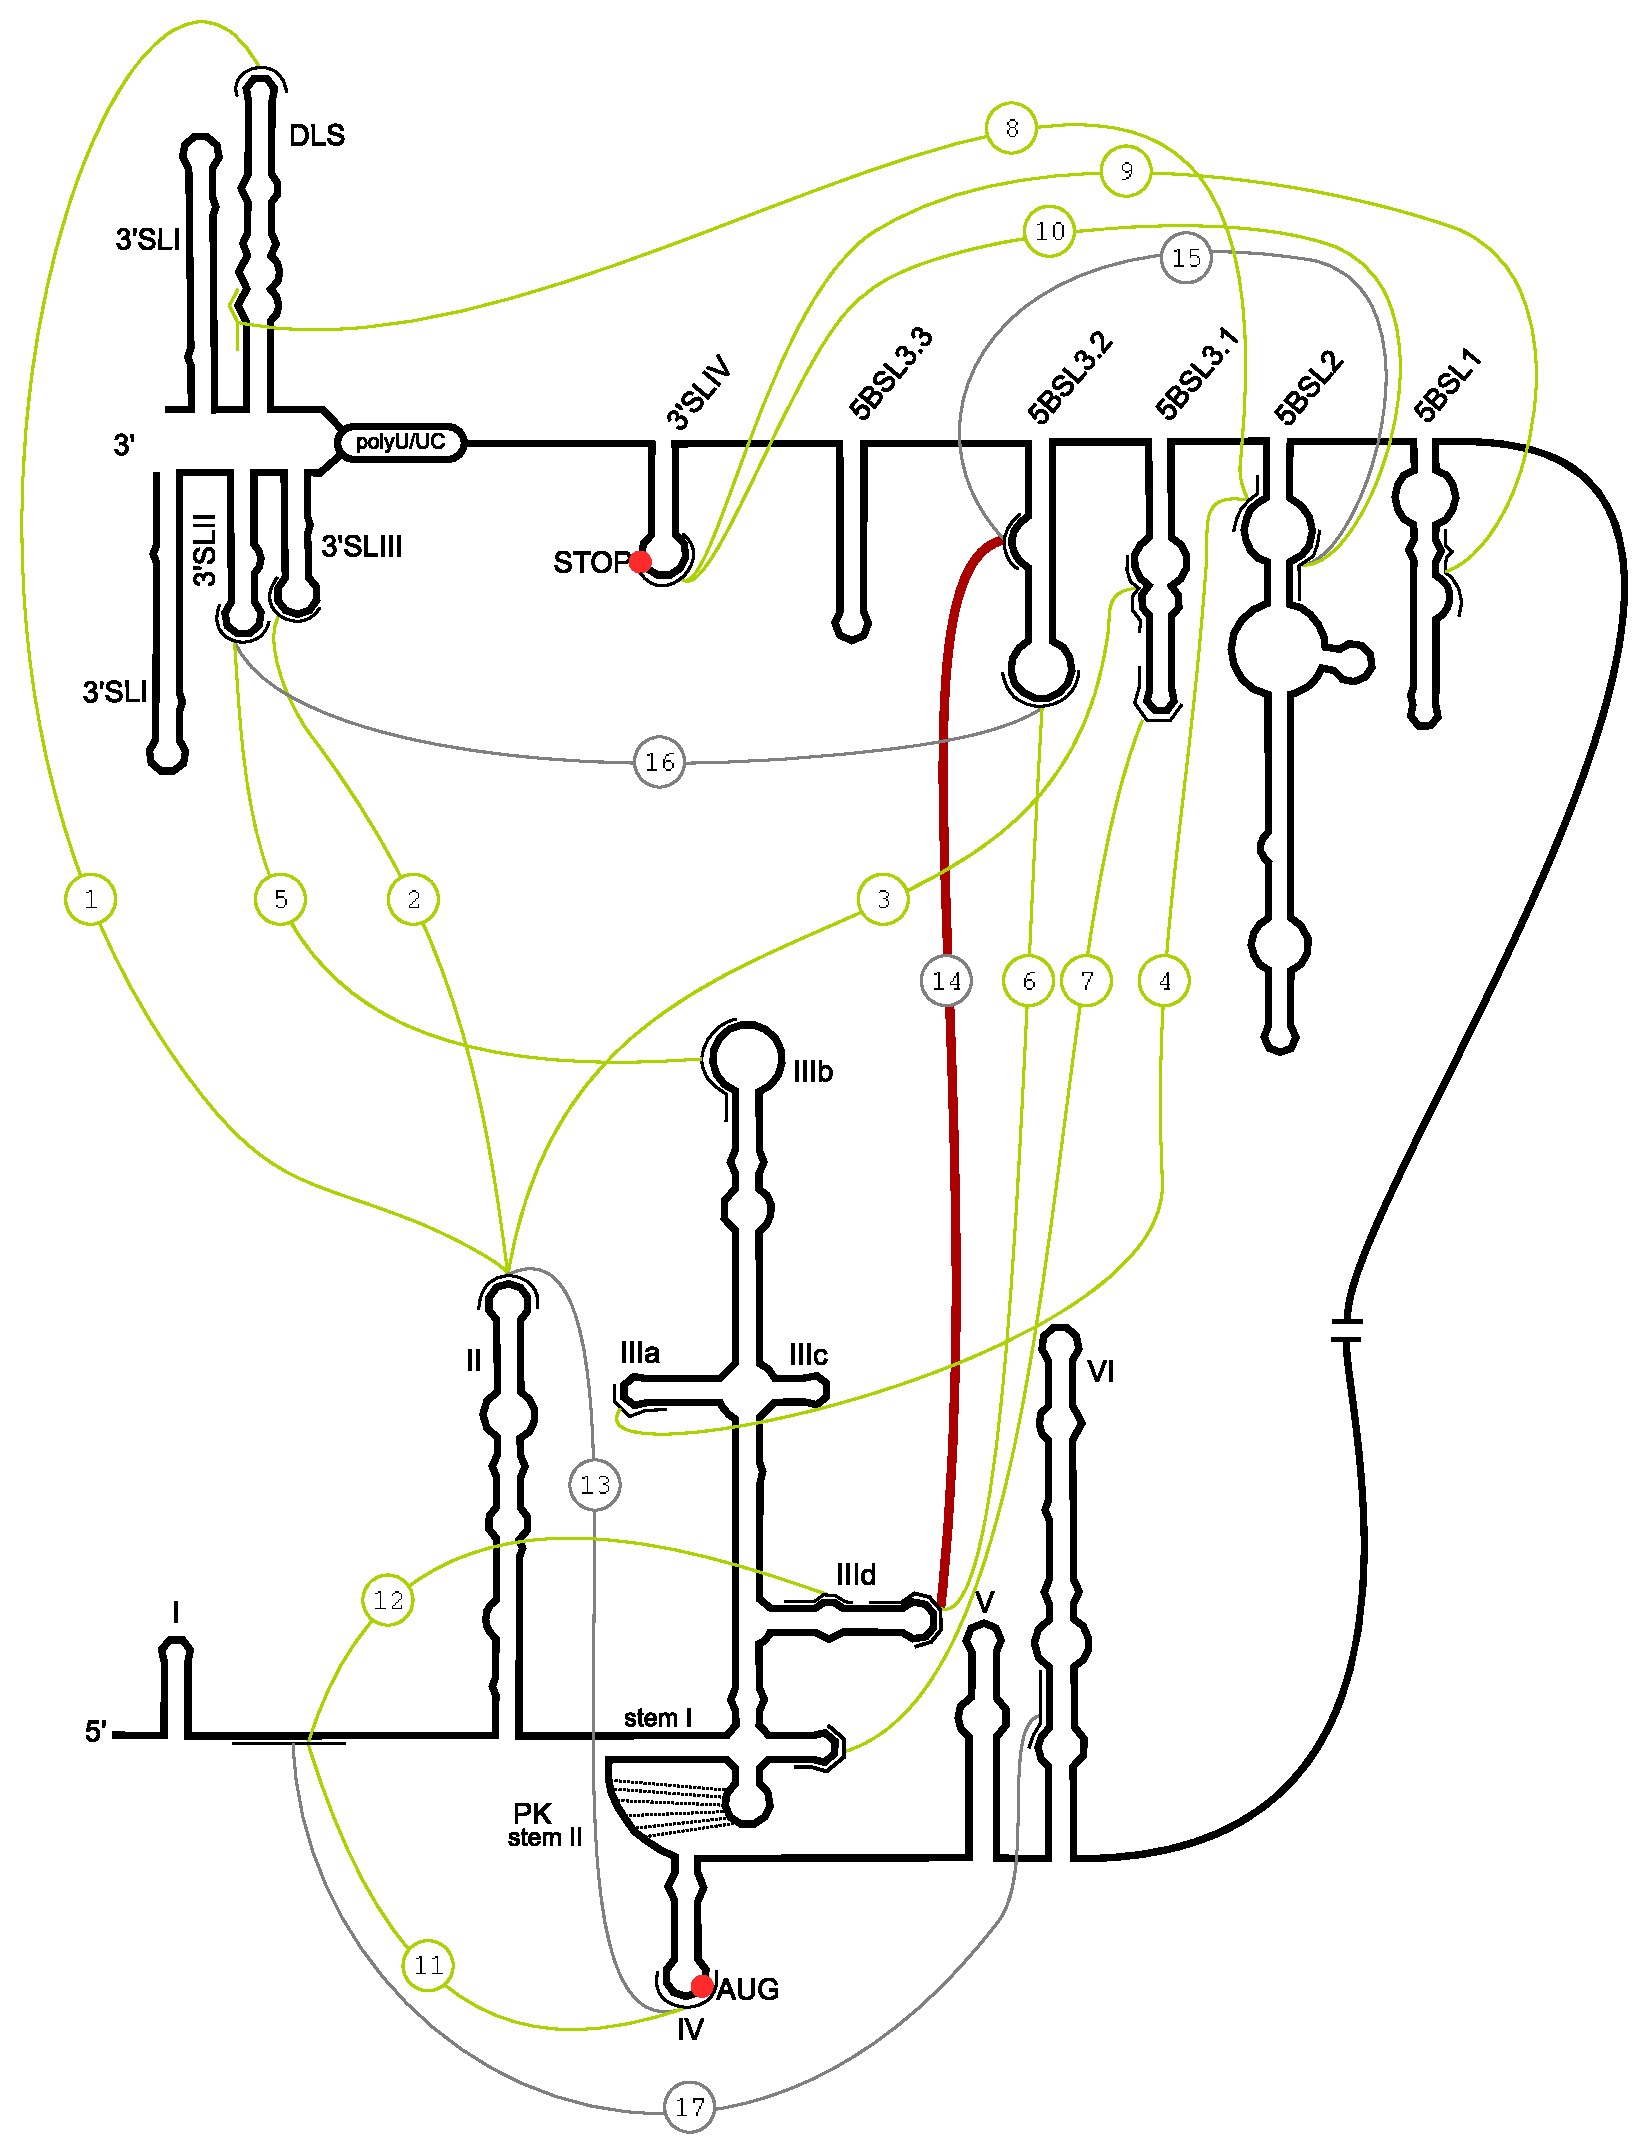
\includegraphics[height=0.7\textheight]{figures/long_range_hcv_trans.pdf}\\%
  \tiny{Fricke, M.~\textit{et al.}~(2015).~Conserved RNA secondary structures and long-range interactions in hepatitis C viruses. RNA, http://doi.org/10.1261/rna.049338.114}%
  }
  \only<3> {
  \centering
  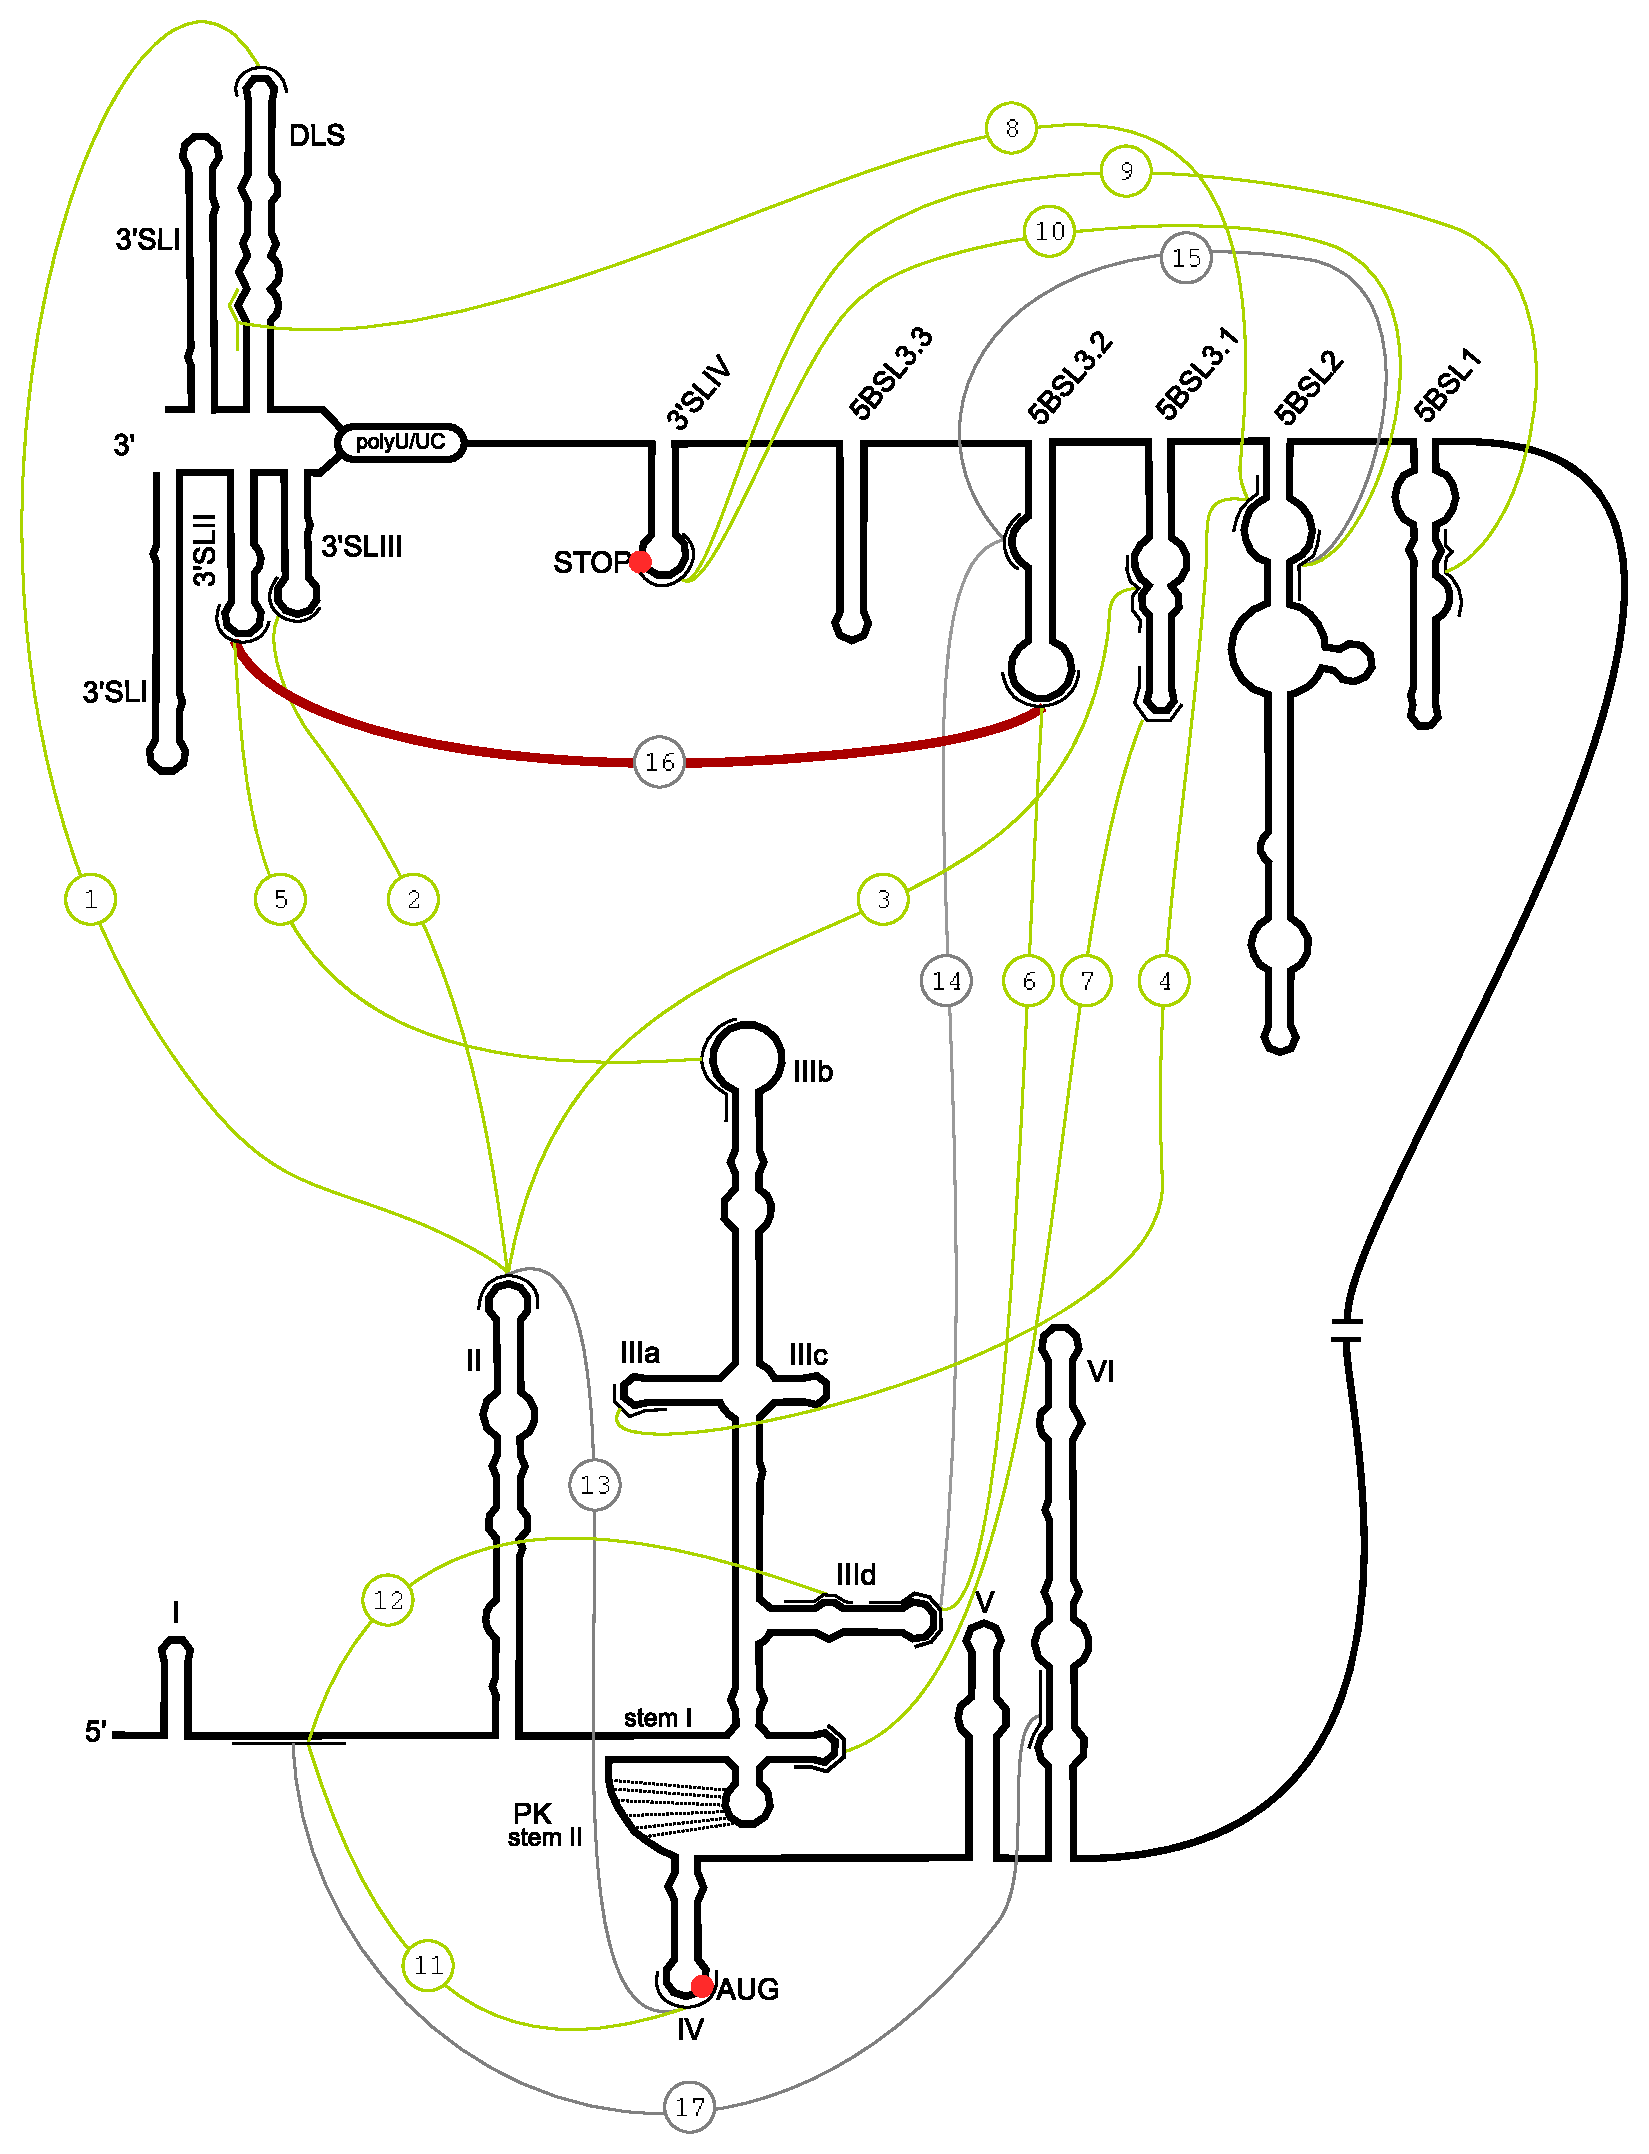
\includegraphics[height=0.7\textheight]{figures/long_range_hcv_repli.pdf}\\%
  \tiny{Fricke, M.~\textit{et al.}~(2015).~Conserved RNA secondary structures and long-range interactions in hepatitis C viruses. RNA, http://doi.org/10.1261/rna.049338.114}% 
  }
\end{overlayarea}
  \column{0.4\textwidth}
  \vspace{-5cm}
  \begin{itemize}
      \item<1-> Hepatitis C virus: (+)ssRNA
      \item<1-> around 9\,kb in size\\[2em]
      \item<2-> Initiation of Translation
      \item<3-> Initiation of Replication
    \end{itemize}
  \end{columns} 
\end{frame}

\begin{frame}[c]{}
  \begin{block}{Exercise:}
    Take any LRI from HCV, described in the following paper, and try to reconstruct / predict it with the ViennaRNA package.\\[2em]
    \tiny{Fricke, M.~\textit{et al.}~(2015).~Conserved RNA secondary structures and long-range interactions in hepatitis C viruses. RNA, http://doi.org/10.1261/rna.049338.114}%
  \end{block}
\end{frame}

% Backup Slides. Using this macro, you'd get a slide number for each
% backup slide without increasing the maximum slide numbers of the original presentation.
% However, for this, the framenumber has to be inserted - which isn't in the template by default
\beginbackup

% \begin{frame}[c]\frametitle{Coffee Break}
%   \begin{figure}[htbp]
%     \centering
%     
\includegraphics[width=0.65\textwidth]{coffeebreak.png}
%   \end{figure}
% \end{frame}

\backupend

\end{document}